 
\chapter{Asymptotic Inference in OLS: the Eicker--Huber--White (EHW) robust standard error}\label{chapter::EHW}
  \chaptermark{EHW standard error in OLS}




\section{Motivation}
Standard software packages, for example, \ri{R}, report the point estimator,
standard error, and $p$-value for each coordinate of $\beta$ based
on the Normal linear model:
\[
Y=X\beta+\varepsilon\sim\N(X\beta,\sigma^{2}I_{n}).
\]
Statistical inference based on this model is finite-sample exact.
However, the assumptions of this model are extremely strong: the functional
form is linear, the error terms are additive with distributions not
dependent on $X$, and the error terms are IID Normal with the
same variance. If we do not believe some of these assumptions, can we still
trust the associated statistical inference? Let us start with some simple numerical examples, with the \ri{R} code in \ri{code6.1.R}. 


\subsection{Numerical examples}

The  first one is the ideal Normal linear model:

\begin{lstlisting}
> library(car)
> n     = 200
> x     = runif(n, -2, 2)
> beta  = 1
> xbeta = x*beta 
> Simu1  = replicate(5000,
+                   {y = xbeta + rnorm(n)
+                   ols.fit = lm(y ~ x)
+                   c(summary(ols.fit)$coef[2, 1:2],
+                     sqrt(hccm(ols.fit)[2, 2]))
+                   })
\end{lstlisting}

In the above, we generate outcomes from a simple linear model $y_i = x_i + \varepsilon_i$ with $\varepsilon_i\iidsim \N(0,\sigma^2=1)$. Over 5000 replications of the data, we computed the OLS coefficient $\hat{\beta}$ of $x_i$ and reported two standard errors. One is the standard error discussed in Chapter \ref{chapter::normal-linear-model} under the Normal linear model, which is also the default choice of the \ri{lm} function of \ri{R}. The other one, computed by the \ri{hccm} function in the \ri{R} package \ri{car}, will be the main topic of this chapter. The $(1,1)$ the panel of
Figure \ref{fig::simulation-nonnormal-heteroskedasticity} shows the histogram of the estimator and reports the standard error (se0), as well as two estimated standard errors (se1 and se2). The distribution of $\hat{\beta}$ is symmetric and bell-shaped around the true parameter 1, and the estimated standard errors are close to the true one. 

To investigate the impact of Normality, we change the error terms to be IID exponential with mean 1 and variance 1. 

\begin{lstlisting}
> Simu2  = replicate(5000,
+                   {y = xbeta + rexp(n)
+                   ols.fit = lm(y ~ x)
+                   c(summary(ols.fit)$coef[2, 1:2],
+                     sqrt(hccm(ols.fit)[2, 2]))
+                   })
\end{lstlisting}

The $(1,2)$ panel of Figure \ref{fig::simulation-nonnormal-heteroskedasticity} corresponds to this setting. With non-Normal errors, $\hat{\beta}$ is still symmetric and bell-shaped around the true parameter 1, and the estimated standard errors are close to the true one. So the Normality of the error terms does not seem to be a crucial assumption for the validity of the inference procedure under the Normal linear model. 



We then generate errors from Normal with variance depending on $x$:
\begin{lstlisting}
> Simu3  = replicate(5000,
+                   {y = xbeta + rnorm(n, 0, abs(x))
+                   ols.fit = lm(y ~ x)
+                   c(summary(ols.fit)$coef[2, 1:2],
+                     sqrt(hccm(ols.fit)[2, 2]))
+                   })
\end{lstlisting}
The $(2,1)$ panel of Figure \ref{fig::simulation-nonnormal-heteroskedasticity} corresponds to this setting. With heteroskedastic Normal errors, $\hat{\beta}$ is symmetric and bell-shaped around the true parameter 1, se2 is close to se0, but se1 underestimates se0. So the heteroskedasticity of the error terms does not change the Normality of the OLS estimator dramatically, although the statistical inference discussed in Chapter \ref{chapter::normal-linear-model} can be invalid. 
 
 
Finally, we generate heteroskedastic non-Normal errors:
\begin{lstlisting}
> Simu4  = replicate(5000,
+                   {y = xbeta + runif(n, -x^2, x^2)
+                   ols.fit = lm(y ~ x)
+                   c(summary(ols.fit)$coef[2, 1:2],
+                     sqrt(hccm(ols.fit)[2, 2]))
+                   })
\end{lstlisting} 
The  $(2,2)$ panel of Figure \ref{fig::simulation-nonnormal-heteroskedasticity} corresponds to this setting, which has a similar pattern as the $(2,1)$ panel. So the Normality of the error terms is not crucial, but the homoskedasticity is. 



\begin{figure}[t]
\centering
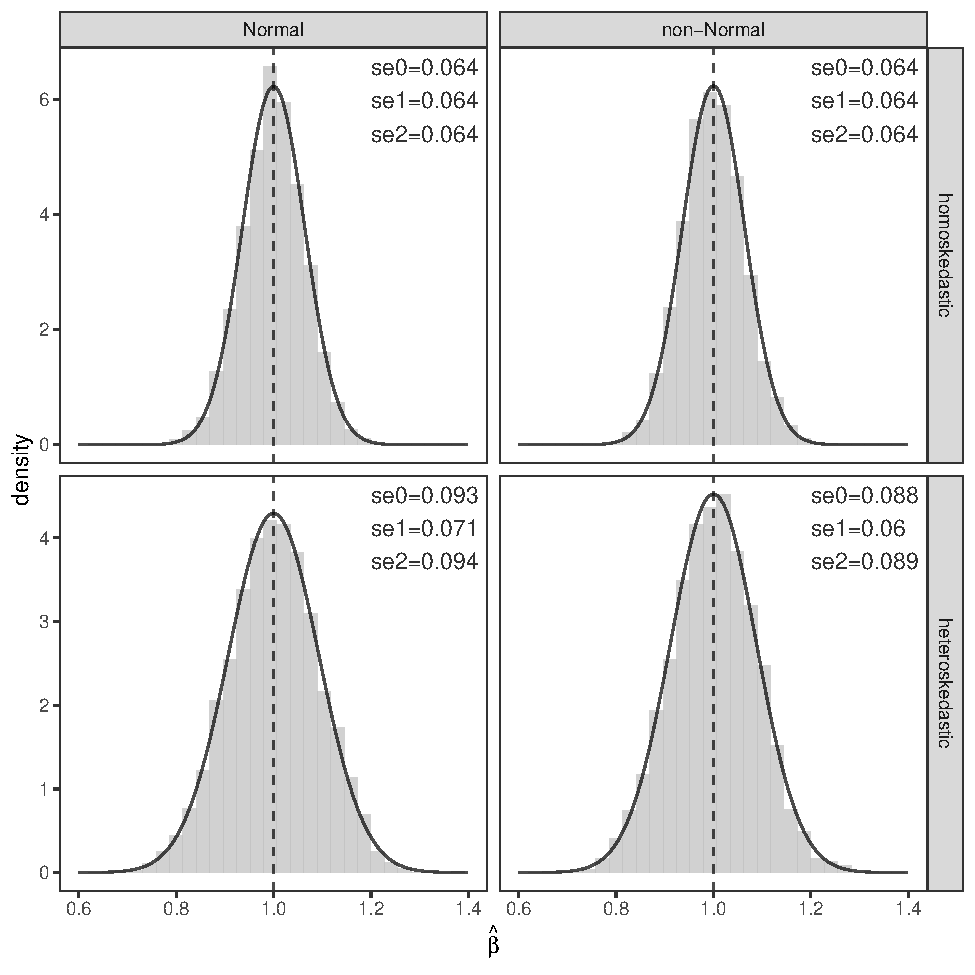
\includegraphics[width=0.98\textwidth]{figures/asymptoticinference_ggplot.pdf}
\caption{Simulation with 5000 replications: ``se0'' denotes the true standard error of $\hat{\beta}$, ``se1'' denotes the estimated standard error based on the homoskedasticity assumption, and ``se2'' denotes the Eicker--Huber--White standard error allowing for heteroskedasticity. The density curves are Normal with mean 1 and standard deviation se0.}
\label{fig::simulation-nonnormal-heteroskedasticity}
\end{figure}



\subsection{Goal of this chapter}

In this chapter, we will still impose the linearity assumption, but
relax the distributional assumption on the error terms. We assume the following heteroskedastic linear model.


\begin{assumption}
[Heteroskedastic linear model]
\label{assume::heteroskedasticity-lm}
We have
\[
y_{i}=x_{i}^{\T}\beta+\varepsilon_{i},
\]
where the $\varepsilon_{i}$'s are independent
with mean zero and variance $\sigma_{i}^{2}$ $(i=1,\ldots,n)$.
The design matrix $X$ is fixed with linearly independent column vectors, and $(\beta,\sigma^{2}_1, \ldots, \sigma^2_n)$
are unknown parameters. 
\end{assumption}


 Because
the error terms can have different variances, they are not IID
in general under the heteroskedastic linear model. Their variances can be functions of the $x_{i}$'s, and
the variances $\sigma_{i}^{2}$ are $n$ free unknown numbers. Again, treating the
$x_{i}$'s as fixed is not essential, because we can condition on
them if they are random. Without imposing Normality on the error terms,
we cannot determine the finite sample exact distribution of the OLS
estimator. This chapter will use the asymptotic analysis,
assuming that the sample size $n$ is large so that certain limiting
theorems hold. 

The asymptotic analysis later will show that if the error terms are
homoskedastic, i.e., $\sigma_{i}^{2}=\sigma^{2}$ for all $i=1,\ldots,n$,
we can still trust the statistical inference discussed in Chapter \ref{chapter::normal-linear-model} based on the Normal
linear model as long the central limit theorem (CLT) for the OLS estimator
holds as $n\rightarrow\infty$. If the error terms are heteroskedastic,
i.e., their variances are different, we must adjust the standard
error with the so-called Eicker--Huber--White heteroskedasticity robust standard error.
I will give the technical details below. 
If you are unfamiliar with the asymptotic analysis, please first review the basics in Chapter \ref{chapter::limiting-theorems}. 


\section{Consistency of OLS}


Under the heteroskedastic linear model,  the OLS estimator $\hat{\beta}$ is still unbiased for $\beta$ because the error terms have to mean zero. Moreover, we can show that it is consistent
for $\beta$ with large $n$ and some regularity conditions. We start
with a useful lemma.
\begin{lemma}
\label{lem:The-OLS-estimator}
Under Assumption \ref{assume::heteroskedasticity-lm}, the OLS estimator has the
representation
$
\hat{\beta}-\beta=\ B_{n}^{-1} \xi_n,
$
where
\begin{eqnarray*}
B_{n} &=& n^{-1}\sumn x_{i}x_{i}^{\T},\\ 
\xi_n &=& n^{-1}\sumn x_{i}\varepsilon_{i}
\end{eqnarray*}
\end{lemma}


\begin{myproof}{Lemma}{\ref{lem:The-OLS-estimator}}
Since $y_{i}=x_{i}^{\T}\beta+\varepsilon_{i}$, we have

\begin{align*}
\hat{\beta} & =B_{n}^{-1}n^{-1}\sumn x_{i}y_{i}\\
 & =B_{n}^{-1}n^{-1}\sumn x_{i}(x_{i}^{\T}\beta+\varepsilon_{i})\\
 & =B_{n}^{-1}B_{n}\beta+B_{n}^{-1}n^{-1}\sumn x_{i}\varepsilon_{i}\\
 & =\beta+ B_{n}^{-1}n^{-1}\sumn x_{i}\varepsilon_{i}.
\end{align*}
\end{myproof}



In the representation of Lemma \ref{lem:The-OLS-estimator}, $B_n$ is fixed and $\xi_n$ is random. Since $E(\xi_n) = 0$, we know that $E(\hat{\beta})=\beta$, so the OLS estimator is unbiased. Moreover, 
\begin{eqnarray*}
\cov(\xi_n)  
&=&  \cov\left( n^{-1}\sumn x_{i}\varepsilon_{i} \right)   \\
&=& n^{-2} \sumn \sigma_{i}^{2}x_{i}x_{i}^{\T} \\
&=&  M_n/n,
\end{eqnarray*}
where
$$
M_{n}=n^{-1}\sumn\sigma_{i}^{2}x_{i}x_{i}^{\T}.
$$
So the covariance of the OLS estimator is 
$$
\cov(\hat{\beta})=n^{-1}B_{n}^{-1}M_{n}B_{n}^{-1}.
$$
It has a sandwich form, justifying
the choice of notation $B_n$ for the ``bread'' and $M_n$ for the ``meat.'' 


Intuitively, if $B_{n}$ and $M_{n}$ have finite limits, then the
covariance of $\hat{\beta}$ shrinks to zero with large $n$, implying
that $\hat{\beta}$ will concentrate near its mean $\beta$. This
is the idea of consistency, formally stated below. 
\begin{assumption}
\label{assume::ols-basic-asymptotic-conditions}
$B_{n}\rightarrow B$ and $M_{n}\rightarrow M$
where $B$ and $M$ are finite with $B$ invertible.
\end{assumption}

\begin{theorem}
\label{thm:consistencyofOLS} Under Assumptions \ref{assume::heteroskedasticity-lm} and \ref{assume::ols-basic-asymptotic-conditions}, we have $\hat{\beta}\rightarrow\beta$
in probability.
\end{theorem}


\begin{myproof}{Theorem}{\ref{thm:consistencyofOLS}}
We only need to show that $ \xi_n \rightarrow0$
in probability. It has mean zero and covariance matrix $M_{n}/n$,
so it converges to zero in probability using Proposition \ref{prop::markov-lln} in Chapter \ref{chapter::limiting-theorems}. 
\end{myproof}

\section{Asymptotic Normality of the OLS estimator}

Intuitively, $ \xi_n$ is the sample average
of some independent terms, and therefore, the classic Lindberg--Feller
theorem guarantees that it enjoys a CLT under some regularity conditions.
Consequently, $\hat{\beta}$ also enjoys a CLT with mean $\beta$
and covariance matrix $n^{-1}B_{n}^{-1}M_{n}B_{n}^{-1}.$ The asymptotic results in this chapter require rather tedious regularity conditions. I give them for generality, and they hold automatically if we are willing to assume that the covariates and error terms are all bounded by a constant not depending on $n$. These general conditions are basically moment conditions required by the law of large numbers and CLT.  You do not have to pay too much attention to the conditions when you first read this chapter. 




The CLT
relies on an additional condition on a higher-order moment 
\[
d_{2+\delta,n}=n^{-1}\sumn\|x_{i}\|^{2+\delta}E(\varepsilon_{i}^{2+\delta}).
\]

\begin{theorem}
\label{thm:clt-ols} Under Assumptions \ref{assume::heteroskedasticity-lm} and \ref{assume::ols-basic-asymptotic-conditions}, if there exist
a $\delta>0$ and $C>0$ not depending on $n$ such that $d_{2+\delta,n} \leq C$,
then 
$$
\sqrt{n}(\hat{\beta}-\beta)\rightarrow\N(0,B^{-1}MB^{-1})
$$
in distribution. 
\end{theorem}


\begin{myproof}{Theorem}{\ref{thm:clt-ols}}
The key is to show the CLT for $ \xi_n$, and the CLT for $\hat{\beta}$ holds due to the Slutsky's Theorem; see Chapter \ref{chapter::limiting-theorems} for a review. Define 
\[
z_{n,i}=n^{-1/2}x_{i}\varepsilon_{i},\qquad(i=1,\ldots,n)
\]
with mean zero and finite covariance, and we need to verify the two conditions required by the Lindeberg--Feller CLT stated as Proposition \ref{prop::lf-clt} in Chapter \ref{chapter::limiting-theorems}. First, the Lyapunov condition holds because
\begin{align*}
\sumn E\left(  \|z_{n,i}\|^{2+\delta} \right) 
& =\sumn E\left(  n^{-(2+\delta)/2}\|x_{i}\|^{2+\delta}\varepsilon_{i}^{2+\delta}  \right)\\
 & =n^{-\delta/2} \times n^{-1}\sumn\|x_{i}\|^{2+\delta}E(\varepsilon_{i}^{2+\delta}) \\
 & =n^{-\delta/2} \times  d_{2+\delta,n} \rightarrow0.
\end{align*}
Second, 
\begin{eqnarray*}
\sumn\cov(z_{n,i})  &=&  n^{-1}\sumn\sigma_{i}^{2}x_{i}x_{i}^{\T} \\
&=& M_{n}\rightarrow M.
\end{eqnarray*}
So the Lindberg--Feller CLT implies that $n^{-1/2}\sumn x_{i}\varepsilon_{i}=\sumn z_{n,i}\rightarrow\N(0,M)$
in distribution. 
\end{myproof}







\section{Eicker--Huber--White standard error}


\subsection{Sandwich variance estimator}
The CLT in Theorem \ref{thm:clt-ols} shows that 
\[
\hat{\beta}\asim\N(\beta,n^{-1}B^{-1}MB^{-1}),
\]
where $\asim$ denotes ``approximation in distribution.'' However,
the asymptotic covariance is unknown, and we need to use the data
to construct a reasonable estimator for statistical inference. It
is relatively easy to replace $B$ with its sample analog $B_{n}$,
but
\[
\tilde{M}_{n}=n^{-1}\sumn\varepsilon_{i}^{2}x_{i}x_{i}^{\T}
\]
as the sample analog for $M$ is not directly useful because the error
terms are unknown either. It is natural to use $\hat{\varepsilon}_{i}^{2}$
to replace $\varepsilon_{i}^{2}$ to obtain the following estimator
for $M$: 
\[
\hat{M}_{n}=n^{-1}\sumn\hat{\varepsilon}_{i}^{2}x_{i}x_{i}^{\T}.
\]

Although each $\hat{\varepsilon}_{i}^{2}$ is a poor estimator for
$\sigma_{i}^{2}$, the sample average $\hat{M}_{n}$ turns out to
be well-behaved with large $n$ and the regularity conditions below. 


\begin{theorem}\label{thm::ehw-fixeddesign-consistency}
Under Assumptions \ref{assume::heteroskedasticity-lm} and \ref{assume::ols-basic-asymptotic-conditions}, 
we have $\hat{M}_{n}\rightarrow M$ in probability
if
\begin{equation}
\label{thm::ehw-consistency}
n^{-1}\sumn\var(\varepsilon_{i}^{2})x_{ij_1}^2 x_{ij_2}^2,\quad
n^{-1}\sumn x_{ij_{1}}x_{ij_{2}}x_{ij_{3}}x_{ij_{4}} ,\quad
n^{-1}\sumn\sigma_{i}^{2}x_{ij_{1}}^{2}x_{ij_{2}}^{2}x_{ij_{3}}^{2}
\end{equation}
are bounded from above by a constant $C$ not depending on $n$ for any $j_{1},j_{2},j_{3},j_{4}=1,\ldots,p$. 
%\begin{align}
%n^{-1}\sumn\var(\varepsilon_{i}^{2})x_{ij_1}^2 x_{ij_2}^2  & \rightarrow c_{j_1 j_2} < \infty  ,\label{eq:condtion1}\\
%n^{-1}\sumn x_{ij_{1}}x_{ij_{2}}x_{ij_{3}}x_{ij_{4}} & \rightarrow c_{j_1j_2j_3j_4} < \infty ,\label{eq:condition2}\\
%n^{-1}\sumn\sigma_{i}^{2}x_{ij_{1}}^{2}x_{ij_{2}}^{2}x_{ij_{3}}^{2} & \rightarrow c_{j_1 j_2 j_3} < \infty,\label{eq:condition3}
%\end{align}
%for any $j_{1},j_{2},j_{3},j_{4}=1,\ldots,p$, then $\hat{M}_{n}\rightarrow M$ in probability. 
\end{theorem}
%
\begin{myproof}{Theorem}{\ref{thm::ehw-fixeddesign-consistency}}
Assumption \ref{assume::ols-basic-asymptotic-conditions} ensures that $\hat{\beta}\rightarrow\beta$
in probability by Theorem \ref{thm:consistencyofOLS}. Markov's inequality and the boundedness of the first term in \eqref{thm::ehw-consistency}
ensure that $\tilde{M}_{n}-M_{n}\rightarrow0$ in probability. So
we only need to show that $\hat{M}_{n}-\tilde{M}_{n}\rightarrow0$
in probability. The $(j_{1},j_{2})$th element of their difference
is
\begin{align*}
(\hat{M}_{n}-\tilde{M}_{n})_{j_{1},j_{2}} & =n^{-1}\sumn\hat{\varepsilon}_{i}^{2}x_{i,j_{1}}x_{i,j_{2}}-n^{-1}\sumn\varepsilon_{i}^{2}x_{i,j_{1}}x_{i,j_{2}}\\
 & =n^{-1}\sumn\left[\left(\varepsilon_{i}+x_{i}^{\T}\beta-x_{i}^{\T}\hat{\beta}\right)^{2}-\varepsilon_{i}^{2}\right]x_{i,j_{1}}x_{i,j_{2}}\\
 & =n^{-1}\sumn\left[\left(x_{i}^{\T}\beta-x_{i}^{\T}\hat{\beta}\right)^{2}+2\varepsilon_{i}\left(x_{i}^{\T}\beta-x_{i}^{\T}\hat{\beta}\right)\right]x_{i,j_{1}}x_{i,j_{2}}\\
 & =(\beta-\hat{\beta})^{\T}n^{-1}\sumn x_{i}x_{i}^{\T}x_{i,j_{1}}x_{i,j_{2}}(\beta-\hat{\beta}) \\
 & \quad +2(\beta-\hat{\beta})^{\T}n^{-1}\sumn x_{i}x_{i,j_{1}}x_{i,j_{2}}\varepsilon_{i}.
\end{align*}
It converges to zero in probability because the first term converges
to zero due to the boundedness of the second term in \eqref{thm::ehw-consistency}, and the second term
converges to zero in probability due to Markov's inequality and the boundedness of the third term in \eqref{thm::ehw-consistency}. 
\end{myproof}



The final variance estimator for $\hat{\beta}$ is 
\[
\hat{V}_{\textsc{ehw}}=n^{-1}\left(n^{-1}\sumn x_{i}x_{i}^{\T}\right)^{-1}\left(n^{-1}\sumn\hat{\varepsilon}_{i}^{2}x_{i}x_{i}^{\T}\right)\left(n^{-1}\sumn x_{i}x_{i}^{\T}\right)^{-1},
\]
 which is called the Eicker--Huber--White (EHW) heteroskedasticity robust covariance matrix.
In matrix form, it equals 
\[
\hat{V}_{\textsc{ehw}} =(X^{\T}X)^{-1}(X^{\T}\hat{\Omega}X)(X^{\T}X)^{-1},
\]
where $\hat{\Omega}=\text{diag}\left\{ \hat{\varepsilon}_{1}^{2},\ldots,\hat{\varepsilon}_{n}^{2}\right\} .$ 
\citet{eicker1967limit} first proposed to use $\hat{V}_{\textsc{ehw}} $.  \citet{white::1980} popularized it in economics which has been influential in empirical research.  Related estimators appeared in many other contexts of statistics.
\citet{cox1961tests} and \citet{huber::1967} discussed the sandwich variance in the context of misspecified parametric models; see Section \ref{sec::mle}. 
\citet{fuller1975regression} proposed a more general form of $\hat{V}_{\textsc{ehw}} $ in the context of survey sampling. 
The square root of the diagonal terms of $\hat{V}_{\textsc{ehw}} $, denoted by $\hat{\text{se}}_{\textsc{ehw},j}\ (j=1,\ldots,p)$, are called the heteroskedasticity-consistent standard errors, heteroskedasticity-robust standard errors, White standard errors, Huber--White standard errors, or Eicker--Huber--White standard errors, among many other names. 

We can conduct statistical inference based on Normal approximations. For example, we can test linear hypotheses based on
$$
\hat{\beta} \asim \N(\beta,  \hat{V}_{\textsc{ehw}}  ),
$$
and in particular, we can infer each element of the coefficient based on 
$$
\hat{\beta}_j \asim \N(\beta_j, \hat{\text{se}}_{\textsc{ehw}, j}^2 ).
$$  



\subsection{Other ``HC'' standard errors}
\label{sec::HCs}


Statistical inference based on the EHW standard error relaxes the parametric assumptions of the Normal linear model. However, its validity relies strongly on the asymptotic argument. At finite samples, it can have poor behaviors. 
Since \citet{white::1980} published his paper, several modifications of $\hat{V}$ appeared aiming for better finite-sample properties. I summarize them below. They all rely on the $h_{ii}$'s, which are the diagonal elements of the projection matrix $H$ and called the {\it leverage scores}. Define
\[
\hat{V}_{\textsc{ehw},k} = n^{-1}\left(n^{-1}\sumn x_{i}x_{i}^{\T}\right)^{-1}\left(n^{-1}\sumn\hat{\varepsilon}_{i,k}^{2}x_{i}x_{i}^{\T}\right)\left(n^{-1}\sumn x_{i}x_{i}^{\T}\right)^{-1},
\]
where  
\[
\hat{\varepsilon}_{i,k}=\begin{cases}
\hat{\varepsilon}_{i}, & (k=0, \text{ HC}0); \\
\hat{\varepsilon}_{i}\sqrt{\frac{n}{n-p},} & (k=1, \text{ HC}1) ; \\
\hat{\varepsilon}_{i}/\sqrt{1-h_{ii}}, & (k=2, \text{ HC}2) ; \\
\hat{\varepsilon}_{i}/(1-h_{ii}), & (k=3, \text{ HC}3); \\
\hat{\varepsilon}_{i}/(1-h_{ii})^{\min\left\{ 2,nh_{ii}/(2p)\right\} }, & (k=4, \text{ HC}4).
\end{cases}
\]
The HC1 correction is similar to the degrees of freedom correction in the OLS covariance estimator. The HC2 correction was motivated by the unbiasedness of covariance when the error terms have the same variance; see Problem \ref{hw::ehw-unbiased-hc2} for more details. The HC3 correction was motivated by a method called {\it jackknife} which will be discussed in Chapter \ref{chapter::leave-one-out}. This version appeared even early than  \citet{white::1980}; see \citet{miller1974unbalanced}, \citet{hinkley1977jackknifing}, and \citet{reeds1978jackknifing}. 
I do not have a good intuition for the HC4 correction. 
See \citet{mackinnon1985some}, \citet{long2000using} and \citet{cribari2004asymptotic} for reviews. Using simulation studies, \citet{long2000using} recommended HC3. 





\subsection{Special case with homoskedasticity}
As an important special case with $\sigma_{i}^{2}=\sigma^{2}$ for
all $i=1,\ldots,n$, we have 
\[
M_{n}=\sigma^{2}n^{-1}\sumn x_{i}x_{i}^{\T}=\sigma^{2}B_{n},
\]
which simplifies the covariance of $\hat{\beta}$ to $\cov(\hat{\beta})=\sigma^{2}B_{n}^{-1} / n,$
and the asymptotic Normality to $\sqrt{n}(\hat{\beta}-\beta)\rightarrow\N(0,\sigma^{2}B^{-1})$
in distribution. We have shown that under the Gauss--Markov model,
$\hat{\sigma}^{2}=(n-p)^{-1}\sumn\hat{\varepsilon}_{i}^{2}$ is unbiased
for $\sigma^{2}$. Moreover, $\hat{\sigma}^{2}$ is consistent for
$\sigma^{2}$ under the same condition as Theorem \ref{thm:consistencyofOLS},
justifying the use of 
\[
\hat{V} = 
\hat{\sigma}^{2}\left(\sumn x_{i}x_{i}^{\T}\right)=\hat{\sigma}^{2}\left(X^{\T}X\right)^{-1}
\]
as the covariance estimator. So under homoskedasticity, we can conduct statistical inference based on the following approximate Normality:
\[
\hat{\beta}\asim\N\left(\beta,\hat{\sigma}^{2}\left(X^{\T}X\right)^{-1}\right).
\]
It is slightly different from the inference based on $t$ and $F$ distributions. But with large $n$, the difference is very small.


I will end this section with a formal result on the consistency of
$\hat{\sigma}^{2}.$



\begin{theorem}\label{thm::homoskeda-asymptotic}
Under Assumptions \ref{assume::heteroskedasticity-lm} and \ref{assume::ols-basic-asymptotic-conditions},  we have $\hat{\sigma}^{2}\rightarrow\sigma^{2}$ in probability if 
 $\sigma_{i}^{2}=\sigma^{2}<\infty$ for all $i=1,\ldots,n$ and $n^{-1} \sumn \var(\varepsilon_i^2  ) $ is bounded above by a constant not depending on $n$. 
\end{theorem}

\begin{myproof}{Theorem}{\ref{thm::homoskeda-asymptotic}}
Using Markov's inequality, we can show that $n^{-1}\sumn\varepsilon_{i}^{2}\rightarrow\sigma^{2}$ 
in probability. In addition, $n^{-1}\sumn\hat{\varepsilon}_{i}^{2}$ has the
same probability limit as $\hat{\sigma}^{2}$. So we only need to
show that $n^{-1}\sumn\hat{\varepsilon}_{i}^{2}-n^{-1}\sumn\varepsilon_{i}^{2}\rightarrow0$
in probability. Their difference is
\begin{align*}
&n^{-1}\sumn\hat{\varepsilon}_{i}^{2}-n^{-1}\sumn\varepsilon_{i}^{2} \\
& =n^{-1}\sumn\left\{ \left(\varepsilon_{i}+x_{i}^{\T}\beta-x_{i}^{\T}\hat{\beta}\right)^{2}-\varepsilon_{i}^{2}\right\} \\
 & =n^{-1}\sumn\left\{ \left(x_{i}^{\T}\beta-x_{i}^{\T}\hat{\beta}\right)^{2}+2\left(x_{i}^{\T}\beta-x_{i}^{\T}\hat{\beta}\right)\varepsilon_{i}\right\} \\
 & =(\beta-\hat{\beta})^{\T}n^{-1}\sumn x_{i}x_{i}^{\T}(\beta-\hat{\beta})+2(\beta-\hat{\beta})^{\T}n^{-1}\sumn x_{i}\varepsilon_{i} 
 \\
 &= -(\beta-\hat{\beta})^{\T}n^{-1}\sumn x_{i}x_{i}^{\T}(\beta-\hat{\beta}),
\end{align*}
where the last step follows from Lemma \ref{lem:The-OLS-estimator}. So the difference converges to zero in probability because $\hat{\beta}-\beta\rightarrow0$
in probability by Theorem \ref{thm:consistencyofOLS} and $B_{n}\rightarrow B$ by Assumption \ref{assume::ols-basic-asymptotic-conditions}. 
\end{myproof}
%





\section{Examples}


I use three examples to compare various standard errors for the regression coefficients, with the \ri{R} code in \ri{code6.5.R}. The \ri{car} package contains the \ri{hccm} function that implements the EHW standard errors.  

\begin{lstlisting}
> library("car")
\end{lstlisting}


\subsection{LaLonde experimental data}

First, I revisit the \ri{lalonde} data. In the following analysis,  different standard errors give similar $t$-values. Only \ri{treat} is significant, but all other pretreatment covariates are not. 



\begin{lstlisting}
> library("Matching")
> data(lalonde)
> ols.fit = lm(re78 ~ ., data = lalonde)
> ols.fit.hc0 = sqrt(diag(hccm(ols.fit, type = "hc0")))
> ols.fit.hc1 = sqrt(diag(hccm(ols.fit, type = "hc1")))
> ols.fit.hc2 = sqrt(diag(hccm(ols.fit, type = "hc2")))
> ols.fit.hc3 = sqrt(diag(hccm(ols.fit, type = "hc3")))
> ols.fit.hc4 = sqrt(diag(hccm(ols.fit, type = "hc4")))
> ols.fit.coef =summary(ols.fit)$coef
> tvalues = ols.fit.coef[,1]/
+   cbind(ols.fit.coef[,2], ols.fit.hc0, ols.fit.hc1, 
+         ols.fit.hc2, ols.fit.hc3, ols.fit.hc4)
> colnames(tvalues) = c("ols", "hc0", "hc1", "hc2", "hc3", "hc4")
> round(tvalues, 2)
              ols   hc0   hc1   hc2   hc3   hc4
(Intercept)  0.07  0.07  0.07  0.07  0.07  0.07
age          1.17  1.29  1.28  1.27  1.25  1.25
educ         1.75  2.03  2.00  1.99  1.94  1.92
black       -1.74 -2.00 -1.97 -1.95 -1.91 -1.91
hisp         0.27  0.30  0.30  0.30  0.29  0.29
married     -0.17 -0.17 -0.17 -0.17 -0.16 -0.16
nodegr      -0.02 -0.01 -0.01 -0.01 -0.01 -0.01
re74         1.40  0.98  0.96  0.92  0.87  0.77
re75         0.13  0.14  0.14  0.13  0.13  0.12
u74          1.16  0.89  0.88  0.87  0.85  0.83
u75         -1.05 -0.76 -0.75 -0.75 -0.74 -0.74
treat        2.61  2.49  2.46  2.45  2.41  2.40
\end{lstlisting}


\subsection{Data from  \citet{king2015robust}}
\label{sec::example-ehw-kingdata1}



The following example comes from \citet{king2015robust}. The outcome variable is the multilateral aid flows, and the covariates include log population, log population squared, gross domestic product, former colony status, distance from the Western world, political freedom, military expenditures, arms imports, and the indicators for the years. Different robust standard errors are quite different for some coefficients. 
 

\begin{lstlisting}
> library(foreign)
> dat = read.dta("isq.dta")
> dat = na.omit(dat[,c("multish", "lnpop", "lnpopsq", 
+                      "lngdp", "lncolony", "lndist", 
+                      "freedom", "militexp", "arms", 
+                      "year83", "year86", "year89", "year92")])
> ols.fit = lm(multish ~ lnpop + lnpopsq + lngdp +  lncolony 
+              + lndist + freedom + militexp + arms 
+              + year83 + year86 + year89 + year92, data=dat)
> ols.fit.hc0 = sqrt(diag(hccm(ols.fit, type = "hc0")))
> ols.fit.hc1 = sqrt(diag(hccm(ols.fit, type = "hc1")))
> ols.fit.hc2 = sqrt(diag(hccm(ols.fit, type = "hc2")))
> ols.fit.hc3 = sqrt(diag(hccm(ols.fit, type = "hc3")))
> ols.fit.hc4 = sqrt(diag(hccm(ols.fit, type = "hc4")))
> ols.fit.coef =summary(ols.fit)$coef
> tvalues = ols.fit.coef[,1]/
+   cbind(ols.fit.coef[,2], ols.fit.hc0, ols.fit.hc1, 
+         ols.fit.hc2, ols.fit.hc3, ols.fit.hc4)
> colnames(tvalues) = c("ols", "hc0", "hc1", "hc2", "hc3", "hc4")
> round(tvalues, 2)
              ols   hc0   hc1   hc2   hc3   hc4
(Intercept)  7.40  4.60  4.54  4.43  4.27  4.14
lnpop       -8.25 -4.46 -4.40 -4.30 -4.14 -4.01
lnpopsq      9.56  4.79  4.72  4.61  4.44  4.31
lngdp       -6.39 -6.14 -6.06 -6.01 -5.88 -5.86
lncolony     4.70  4.75  4.69  4.64  4.53  4.47
lndist      -0.14 -0.16 -0.16 -0.16 -0.15 -0.16
freedom      2.25  1.80  1.78  1.75  1.69  1.65
militexp     0.51  0.59  0.59  0.57  0.55  0.52
arms         1.34  1.17  1.15  1.10  1.03  0.91
year83       1.05  0.85  0.84  0.83  0.80  0.79
year86       0.35  0.40  0.39  0.39  0.38  0.38
year89       0.70  0.81  0.80  0.80  0.78  0.79
year92       0.31  0.40  0.40  0.40  0.39  0.40
\end{lstlisting}

However, if we apply the log transformation on the outcome, then all standard errors give similar $t$-values. 

\begin{lstlisting}
> ols.fit = lm(log(multish + 1) ~ lnpop + lnpopsq + lngdp +  lncolony 
+              + lndist + freedom + militexp + arms 
+              + year83 + year86 + year89 + year92, data=dat)
> ols.fit.hc0 = sqrt(diag(hccm(ols.fit, type = "hc0")))
> ols.fit.hc1 = sqrt(diag(hccm(ols.fit, type = "hc1")))
> ols.fit.hc2 = sqrt(diag(hccm(ols.fit, type = "hc2")))
> ols.fit.hc3 = sqrt(diag(hccm(ols.fit, type = "hc3")))
> ols.fit.hc4 = sqrt(diag(hccm(ols.fit, type = "hc4")))
> ols.fit.coef =summary(ols.fit)$coef
> tvalues = ols.fit.coef[,1]/
+   cbind(ols.fit.coef[,2], ols.fit.hc0, ols.fit.hc1, 
+         ols.fit.hc2, ols.fit.hc3, ols.fit.hc4)
> colnames(tvalues) = c("ols", "hc0", "hc1", "hc2", "hc3", "hc4")
> round(tvalues, 2)
              ols   hc0   hc1   hc2   hc3   hc4
(Intercept)  2.96  2.81  2.77  2.72  2.63  2.53
lnpop       -2.87 -2.63 -2.60 -2.54 -2.45 -2.35
lnpopsq      4.21  3.72  3.67  3.59  3.46  3.32
lngdp       -8.02 -7.49 -7.38 -7.38 -7.27 -7.33
lncolony     6.31  6.19  6.11  6.08  5.97  5.95
lndist      -0.16 -0.14 -0.14 -0.14 -0.14 -0.14
freedom      1.47  1.53  1.51  1.50  1.47  1.46
militexp    -0.32 -0.32 -0.31 -0.31 -0.30 -0.29
arms         1.27  1.12  1.10  1.05  0.98  0.86
year83       0.10  0.10  0.10  0.10  0.10  0.10
year86      -0.14 -0.14 -0.14 -0.14 -0.14 -0.14
year89       0.46  0.45  0.44  0.44  0.44  0.44
year92       0.03  0.03  0.03  0.03  0.03  0.03
\end{lstlisting}


  In general, the difference between the OLS and EHW standard errors may be due to the heteroskedasticity or the poor approximation of the linear model. The above two analyses based on the original and transformed outcomes suggest that the linear approximation works better for the log-transformed outcome. 
  We will discuss the issues of transformation and model misspecification later. 


\subsection{Boston housing data}


I also re-analyze the classic Boston housing data \citep{harrison1978hedonic}. The outcome variable is the median value of owner-occupied homes in US dollars 1000, and the covariates include per capita crime rate by town, the proportion of residential land zoned for lots over 25,000 square feet, the proportion of non-retail business acres per town, etc. You can find more details in the R package. In this example, different standard errors yield very different $t$-values. 


\begin{lstlisting}
> library("mlbench")
> data(BostonHousing)
> ols.fit = lm(medv ~ ., data = BostonHousing)
> summary(ols.fit)

Call:
lm(formula = medv ~ ., data = BostonHousing)

Residuals:
    Min      1Q  Median      3Q     Max 
-15.595  -2.730  -0.518   1.777  26.199 

Coefficients:
              Estimate Std. Error t value Pr(>|t|)    
(Intercept)  3.646e+01  5.103e+00   7.144 3.28e-12 ***
crim        -1.080e-01  3.286e-02  -3.287 0.001087 ** 
zn           4.642e-02  1.373e-02   3.382 0.000778 ***
indus        2.056e-02  6.150e-02   0.334 0.738288    
chas1        2.687e+00  8.616e-01   3.118 0.001925 ** 
nox         -1.777e+01  3.820e+00  -4.651 4.25e-06 ***
rm           3.810e+00  4.179e-01   9.116  < 2e-16 ***
age          6.922e-04  1.321e-02   0.052 0.958229    
dis         -1.476e+00  1.995e-01  -7.398 6.01e-13 ***
rad          3.060e-01  6.635e-02   4.613 5.07e-06 ***
tax         -1.233e-02  3.760e-03  -3.280 0.001112 ** 
ptratio     -9.527e-01  1.308e-01  -7.283 1.31e-12 ***
b            9.312e-03  2.686e-03   3.467 0.000573 ***
lstat       -5.248e-01  5.072e-02 -10.347  < 2e-16 ***

Residual standard error: 4.745 on 492 degrees of freedom
Multiple R-squared:  0.7406,	Adjusted R-squared:  0.7338 
F-statistic: 108.1 on 13 and 492 DF,  p-value: < 2.2e-16

> 
> ols.fit.hc0 = sqrt(diag(hccm(ols.fit, type = "hc0")))
> ols.fit.hc1 = sqrt(diag(hccm(ols.fit, type = "hc1")))
> ols.fit.hc2 = sqrt(diag(hccm(ols.fit, type = "hc2")))
> ols.fit.hc3 = sqrt(diag(hccm(ols.fit, type = "hc3")))
> ols.fit.hc4 = sqrt(diag(hccm(ols.fit, type = "hc4")))
> ols.fit.coef =summary(ols.fit)$coef
> tvalues = ols.fit.coef[,1]/
+   cbind(ols.fit.coef[,2], ols.fit.hc0, ols.fit.hc1, 
+         ols.fit.hc2, ols.fit.hc3, ols.fit.hc4)
> colnames(tvalues) = c("ols", "hc0", "hc1", "hc2", "hc3", "hc4")
> round(tvalues, 2)
               ols   hc0   hc1   hc2   hc3   hc4
(Intercept)   7.14  4.62  4.56  4.48  4.33  4.25
crim         -3.29 -3.78 -3.73 -3.48 -3.17 -2.58
zn            3.38  3.42  3.37  3.35  3.27  3.28
indus         0.33  0.41  0.41  0.41  0.40  0.40
chas1         3.12  2.11  2.08  2.05  2.00  2.00
nox          -4.65 -4.76 -4.69 -4.64 -4.53 -4.52
rm            9.12  4.57  4.51  4.43  4.28  4.18
age           0.05  0.04  0.04  0.04  0.04  0.04
dis          -7.40 -6.97 -6.87 -6.81 -6.66 -6.66
rad           4.61  5.05  4.98  4.91  4.76  4.65
tax          -3.28 -4.65 -4.58 -4.54 -4.43 -4.42
ptratio      -7.28 -8.23 -8.11 -8.06 -7.89 -7.93
b             3.47  3.53  3.48  3.44  3.34  3.30
lstat       -10.35 -5.34 -5.27 -5.18 -5.01 -4.93
\end{lstlisting}


The log transformation of the outcome does not remove the discrepancy among the standard errors. In this example, heteroskedasticity seems an important problem. 


\begin{lstlisting}
> ols.fit = lm(log(medv) ~ ., data = BostonHousing)
> summary(ols.fit)

Call:
lm(formula = log(medv) ~ ., data = BostonHousing)

Residuals:
     Min       1Q   Median       3Q      Max 
-0.73361 -0.09747 -0.01657  0.09629  0.86435 

Coefficients:
              Estimate Std. Error t value Pr(>|t|)    
(Intercept)  4.1020423  0.2042726  20.081  < 2e-16 ***
crim        -0.0102715  0.0013155  -7.808 3.52e-14 ***
zn           0.0011725  0.0005495   2.134 0.033349 *  
indus        0.0024668  0.0024614   1.002 0.316755    
chas1        0.1008876  0.0344859   2.925 0.003598 ** 
nox         -0.7783993  0.1528902  -5.091 5.07e-07 ***
rm           0.0908331  0.0167280   5.430 8.87e-08 ***
age          0.0002106  0.0005287   0.398 0.690567    
dis         -0.0490873  0.0079834  -6.149 1.62e-09 ***
rad          0.0142673  0.0026556   5.373 1.20e-07 ***
tax         -0.0006258  0.0001505  -4.157 3.80e-05 ***
ptratio     -0.0382715  0.0052365  -7.309 1.10e-12 ***
b            0.0004136  0.0001075   3.847 0.000135 ***
lstat       -0.0290355  0.0020299 -14.304  < 2e-16 ***

Residual standard error: 0.1899 on 492 degrees of freedom
Multiple R-squared:  0.7896,	Adjusted R-squared:  0.7841 
F-statistic: 142.1 on 13 and 492 DF,  p-value: < 2.2e-16

> 
> ols.fit.hc0 = sqrt(diag(hccm(ols.fit, type = "hc0")))
> ols.fit.hc1 = sqrt(diag(hccm(ols.fit, type = "hc1")))
> ols.fit.hc2 = sqrt(diag(hccm(ols.fit, type = "hc2")))
> ols.fit.hc3 = sqrt(diag(hccm(ols.fit, type = "hc3")))
> ols.fit.hc4 = sqrt(diag(hccm(ols.fit, type = "hc4")))
> ols.fit.coef =summary(ols.fit)$coef
> tvalues = ols.fit.coef[,1]/
+   cbind(ols.fit.coef[,2], ols.fit.hc0, ols.fit.hc1, 
+         ols.fit.hc2, ols.fit.hc3, ols.fit.hc4)
> colnames(tvalues) = c("ols", "hc0", "hc1", "hc2", "hc3", "hc4")
> round(tvalues, 2)
               ols   hc0   hc1   hc2   hc3   hc4
(Intercept)  20.08 14.29 14.09 13.86 13.43 13.13
crim         -7.81 -5.31 -5.24 -4.85 -4.39 -3.56
zn            2.13  2.68  2.64  2.62  2.56  2.56
indus         1.00  1.46  1.44  1.43  1.40  1.41
chas1         2.93  2.69  2.66  2.62  2.56  2.56
nox          -5.09 -4.79 -4.72 -4.67 -4.56 -4.54
rm            5.43  3.31  3.26  3.20  3.10  3.02
age           0.40  0.33  0.32  0.32  0.31  0.31
dis          -6.15 -6.12 -6.03 -5.98 -5.84 -5.82
rad           5.37  5.23  5.16  5.05  4.87  4.67
tax          -4.16 -5.05 -4.98 -4.90 -4.76 -4.69
ptratio      -7.31 -8.84 -8.72 -8.67 -8.51 -8.55
b             3.85  2.80  2.76  2.72  2.65  2.59
lstat       -14.30 -7.86 -7.75 -7.63 -7.40 -7.28
\end{lstlisting}



\section{Final remarks}

The beauty of the asymptotic analysis and the EHW standard error is that they hold under weak parametric assumptions on the error term. We do not need to modify the OLS estimator but only need to modify the covariance estimator. 

However, this framework has limitations. First, the proofs are based on limiting theorems that require the sample size to be infinity. We are often unsure whether the sample size is large enough for a particular application we have. Second, the EHW standard errors can be severely biased and have large variability. Finally, under the heteroskedastic linear model, the Gauss--Markov theorem does not hold, so the OLS can be inefficient. We will discuss possible improvements in Chapter \ref{chapter::WLS}. Finally, unlike Section \ref{sec::prection-normallinear}, we cannot create any reasonable prediction intervals for a future observation $y_{n+1}$ based on $(X,Y, x_{n+1})$ since its variance $\sigma_{n+1}^2$ is fundamentally unknown without further assumptions. 



\section{Homework problems}

\paragraph{Testing linear hypotheses under heteroskedasticity} Under the heteroskedastic linear model, how to test the hypotheses
$$
H_0: c^{\T} \beta = 0,  
$$
for $c\in \mathbb{R}^p$,
and
$$
H_0:  C\beta = 0
$$
for $ C\in \mathbb{R}^{l\times p}$ with linearly independent rows?



\paragraph{Two-sample problem continued}\label{hw08::twosample-ehw}

Continue Problem \ref{hw5::two-sample}. 

\begin{enumerate}
\item Assume that $z_{1},\ldots,z_{m}$ are IID with mean $\mu_{1}$ and
variance $\sigma_{1}^{2}$, and $w_{1},\ldots,w_{n}$ are IID with
mean $\mu_{2}$ and variance $\sigma_{2}^{2}$, and test
$H_0: \mu_{1}=\mu_{2}$. Show that under $H_0$, the following
$t$ statistic has an asymptotically Normal distribution:
\[
t_{\text{unequal}}=\frac{\bar{z}-\bar{w}}{\sqrt{S_{z}^{2}/m+S_{w}^{2}/n}}\rightarrow \N(0,1)
\]
in distribution. 

Remark: 
The name  ``\ri{unequal}'' is motivated by the ``\ri{var.equal}''
parameter of the \ri{R} function \ri{t.test}.

\item We can write the above problem as testing hypothesis $H_{0}:\beta_{1}=0$ in the heteroskedastic linear regression. Based on the EHW standard error, we can compute the $t$ statistic.
Show that it is identical to $t_{\text{unequal}}$ with the HC2 correction.
\end{enumerate}


\paragraph{ANOVA with heteroskedasticity}\label{hw8::anova-ols-hc02}

This is an extension of Problem \ref{hw5:anova-f} in Chapter \ref{chapter::normal-linear-model}. 
Assume $y_i \mid i \in \mathcal{T}_j $ has mean $\beta_j$ and variance $\sigma_j^2$, which can be rewritten as a linear model without the Normality and homoskedasticity. In the process of solving Problem \ref{hw5:anova-f}, you have derived the estimator of the covariance matrix of the OLS estimator under homoskedasticity. Find the  HC0 and HC2 versions of the EHW covariance matrix. Which covariance matrices do you recommend, and why? 

 
 %Hint: The results in Problems \ref{hw3::invariance-ols} and \ref{hw03::invariance-of-H} are useful. 


 
 \paragraph{Invariance of the EHW covariance estimator}
\label{hw08::invariance-ehw01234}



If we transform $X$ to $\tilde{X} = X\Gamma$ where $\Gamma$ is a $p\times p$ non-degenerate matrix, the OLS fit changes from
$$
Y = X\hat{\beta} + \hat{\varepsilon}
$$
to
$$
Y = \tilde{X}\tilde{\beta} + \tilde{\varepsilon},
$$
and the associated EHW covariance estimator changes from $\hat{V}_\textsc{ehw}$ to $\tilde{V}_\textsc{ehw}$. Show that
$$
\hat{V} = \Gamma \tilde{V}  \Gamma^{\T},
$$ 
and the above result holds for HC$j$ $(j=0,1,2,3,4)$. Show that the relationship also holds for the covariance estimator assuming homoskedasticity. 


Hint: You can use the results in Problems \ref{hw3::invariance-ols} and \ref{hw03::invariance-of-H}. 







\paragraph{Breakdown of the equivalence of the $t$-statistics based on the EHW standard error}\label{hw6::t-stat-equivalent-breakdown}


This problem parallels Problem \ref{hw5::t-stat-equivalent}. 


With the data $(x_i, y_i)_{i=1}^n$ where both $x_i$ and $y_i$ are scalars. Run OLS fit of $y_i$ on $(1,x_i)$ to obtain $t_{y\mid x}$, the $t$-statistic of the coefficient of $x_i$, based on the EHW standard error. Run OLS fit of $x_i$ on $(1,y_i)$ to obtain $t_{x\mid y}$, the $t$-statistic of the coefficient of $y_i$, based on the EHW standard error. 

Give a counterexample with $t_{y\mid x} \neq  t_{x\mid y}$.




 
 
\paragraph{Empirical comparison of the standard errors}
\citet{long2000using} reviewed and compared several commonly-used standard errors in OLS. Redo their simulation and replicate their Figures 1--4. They specified more details of their covariate generating process in a technical report \citep{long1998correcting}. 


\paragraph{Robust standard error in practice}
\citet{king2015robust} gave three examples where the EHW standard errors differ from the OLS standard error. I have replicated one example in Section \ref{sec::example-ehw-kingdata1}. Replicate another one using linear regression although the original analysis used Poisson regression. You can find the datasets used by \citet{king2015robust} at Harvard Dataverse (\texttt{https://dataverse.harvard.edu/}). 


\paragraph{Unbiased sandwich variance estimator under the Gauss--Markov model}\label{hw::ehw-unbiased-hc2}

Under the Gauss--Markov model with $\sigma_i^2 = \sigma^2$ for $i=1,\ldots, n$, show that the HC0 version of $\hat{V}_{\textsc{ehw}} $ is biased but the HC2 version of $\tilde{V}_{\textsc{ehw}} $ is unbiased  for $\cov(\hat{\beta})$. 





